\section{Колірні моделі та простори}

Оскільки цифрова електроніка оперує лише дискретною математикою, то над вченими 20 століття постала проблема представлення кольорів у ЕОМ. Основна ідея представлення кольорів прийшла з науки біології та експериментальним шляхом було доведено, що людина є трихроматом \cite{ColorSeing}. Сітчатка ока трихроматів має 3 види рецепторів, що називаються ковбочками, які відповідають за колірний зір. Кожна з цих ковбочок має як параметр деяку довжину хвилі, на яку вона дає максимальний зворотній сигнал.

За історичних обставин склалося так, що еталонним колірним простором є XYZ. Ця колірна модель була запропонована та прийнята організацією CIE ( International Commission on Illumination ) у 1931 році. Саме ця модель є базовою для практично усіх інших колірних моделей.

Експерименти, що були проведені Девідом Райтом та Джоном Гілдом у 1930х роках послужили основою для визначення функції колірної відповідності.

Колір у моделі XYZ задається таким чином:
\begin{equation}
	\begin{split}
		X = \int_{380}^{780} I(\lambda)*x(\lambda) \mathrm{d} \lambda \\
		Y = \int_{380}^{780} I(\lambda)*y(\lambda) \mathrm{d} \lambda \\
		Z = \int_{380}^{780} I(\lambda)*z(\lambda) \mathrm{d} \lambda
	\end{split}
	\label{eq:xyz}
\end{equation}


\begin{figure}[H]
	\centering
	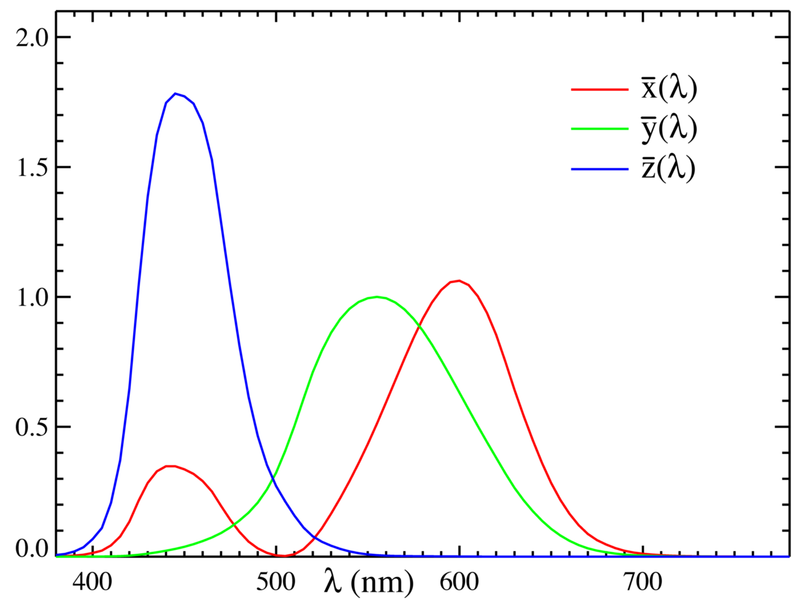
\includegraphics[width=0.7\linewidth]{theory/img/xyz_waves}
	\caption{Функції колірної відповідності}
	\label{fig:xyz_waves}
\end{figure}

Саме ця модель задає правила змішування кольорів та задає обмеження що накладаються на спектральні складові, які мають один колір.

Якщо формально побудувати переріз простору XYZ площиною $ X + Y + Z = const $, то 2 з 3 координат будуть лінійно незалежні і їх можна записати так:

\begin{equation}
	\begin{split}
		x = \frac{X}{X + Y + Z} \\
		y = \frac{Y}{X + Y + Z} \\
		z = \frac{Z}{X + Y + Z}
	\end{split}
	\label{eq:xyz_plate_cut}
\end{equation}

Такий переріз називається хроматичною діаграмою.

\begin{figure}[H]
	\centering
	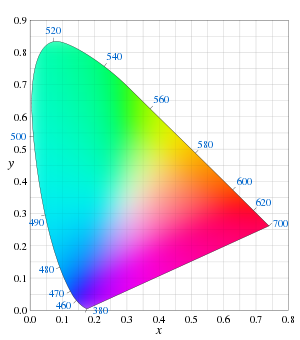
\includegraphics[width=0.5\linewidth]{theory/img/chromatic_diagram}
	\caption{Хроматична діаграма з довжинами хвиль кольорів}
	\label{fig:chromatic_diagram}
\end{figure}

\subsection{RGB}
RGB (скорочено від англ. Red, Green, Blue — червоний, зелений, синій) — адитивна колірна модель, що описує спосіб синтезу кольору, за якою червоне, зелене та синє світло накладаються разом, змішуючись у різноманітні кольори. Широко застосовується в техніці, що відтворює зображення за допомогою випромінення світла.

У даній моделі колір кодуєтся градаціями складових каналів (Red, Green, Blue). Тому за збільшення величини градації котрогось каналу — зростає його інтенсивність під час синтезу.

Кількість градацій кожного каналу залежить від розрядності бітового значення RGB. Зазвичай використовують 24-бітну модель, у котрій визначається по 8 біт на кожен канал, і тому кількість градацій дорівнює 256, що дозволяє закодувати 2563 = 16 777 216  кольорів.

\begin{figure}[H]
	\centering
	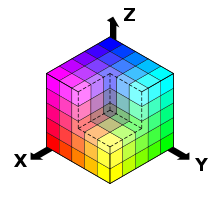
\includegraphics[width=0.7\linewidth]{theory/img/rgb_representation}
	\caption{Тривимірне представлення моделі RGB}
	\label{fig:rgb_representation}
\end{figure}

Колірна модель RGB призначена сприймати, представляти та відображати зображення в електронних системах, таких як телебачення та комп'ютери, хоча її також застосовували у традиційній фотографії. Вже до електронного віку, модель RGB мала за собою серйозну теорію, засновану на сприйнятті кольорів людиною.

Типово приладами із RGB-входом є кольоровий телевізор і відеокамера, сканер і цифровий фотоапарат.

\begin{figure}[H]
	\centering
	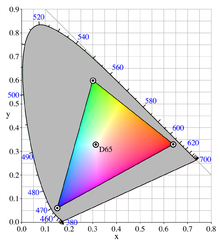
\includegraphics[width=0.7\linewidth]{theory/img/rgb_limitations}
	\caption{Обмеженість моделі по можливості передачі кольору}
	\label{fig:rgb_limitations}
\end{figure}

Переваги моделі:
\begin{enumerate}
	\item Апаратна близкість із монітором, сканером, проектором, іншими пристроями;
	\item Велика кольорова гама, близька до можливостей людського зору;
	\item Доступність багатьох функцій обробки зображення (фільтрів) у програмах растрової графіки;
	\item Невеликий (порівняно до моделі CMYK) обсяг, проте ширший спектр кольорів.
\end{enumerate}
\bigbreak
Недоліки:
\begin{enumerate}
	\item Обмеженість моделі (Рис \ref{fig:rgb_limitations});
	\item Немає явного відділення люмінантної компоненти - для аналізу яскравості пікселя потрібно робити додаткові перетворення.
\end{enumerate}

\subsection{HSV}
HSB — колірна модель, що використовується тільки для оформлення векторних і текстових об'єктів документа. Описує колірний простір, заснований на трьох характеристиках кольору: колірному тоні (Hue), насиченості (Saturation) і яскравості (Brightness).

\begin{itemize}
	\item Hue — колірний тон, (наприклад, червоний, зелений або синьо-блакитний). Варіюється в межах 0-360°, але іноді приводиться до діапазону 0-100 або 0-1. У Windows весь колірний спектр ділиться на 240 відтінків (що можна спостерігати в редакторі палітри MS Paint), тобто тут «Hue» зводиться до діапазону 0-240 (відтінок 240 відсутній, оскільки він дублював би 0).

	\item Saturation — насиченість. Варіюється в межах 0-100 або 0-1. Чим більший цей параметр, тим «чистіший» колір, тому цей параметр іноді називають чистотою кольору. А чим ближчий цей параметр до нуля, тим ближчий колір до нейтрального сірого.
	
	\item Value (значення кольору) або Brightness — яскравість. Також задається в межах 0-100 або 0-1.
\end{itemize}

Модель була створена Елві Реєм Смітом, одним із засновників Pixar, в 1978 році. Вона є нелінійним перетворенням моделі RGB.

\begin{figure}[H]
	\centering
	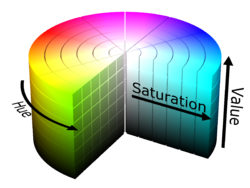
\includegraphics[width=0.7\linewidth]{theory/img/hsv_representation_cylindric}
	\caption{Циліндричне представлення колірного простору}
	\label{fig:hsv_representation_cylindric}
\end{figure}

\begin{figure}[H]
	\centering
	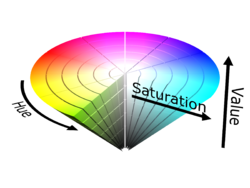
\includegraphics[width=0.7\linewidth]{theory/img/hsv_representation_cone}
	\caption{Конічне представлення колірного простору}
	\label{fig:hsv_representation_cone}
\end{figure}


Колір, представлений в HSV, залежить від пристрою, на який він буде виведений, так як HSV — перетворення моделі RGB, яка теж залежить від пристрою. Для отримання коду кольору, не залежного від пристрою, використовується модель Lab.

\subsection{Lab}

Корірний простір Lab використовує як параметри світлосилу, відношення зеленого до червоного та відношення синього до жовтого. Ці три параметри утворюють тривимірний простір, точки якого відповідають певним кольорам.

Цей колірний простір розроблявся як апаратно-незалежний, тобто він задає кольори без врахування особливостей відтворення кольорів. Має три параметри для опису кольору: світлосила L (англ. Lightness) та два хроматичні параметри. Перший (умовно позначений латинською літерою a) вказує на співвідношення зеленої і червоної складової кольору, другий (позначений літерою b) — співвідношення синьої та жовтої складової.

На відміну від кольорових просторів RGB чи CMYK, які є, по суті, набором апаратних даних для відтворення кольору на папері чи на екрані монітора, Lab однозначно визначає колір. Тому Lab широко використовується в програмному забезпеченні для обробки зображень у якості проміжного кольорового простору, через яке проходить конвертування даних між іншими кольоровими просторами(наприклад, з RGB сканера в CMYK печатного процесу). При цьому особливі властивості Lab зробили редагування в цьому просторі потужним інструментом корекції кольору.

Завдяки характеру визначення кольору в Lab з'являється можливість окремо впливати на яскравість, контраст зображення і на його колір. У багатьох випадках це дозволяє прискорити обробку зображень. Lab надає можливість вибіркового впливу на окремі кольори в зображенні, посилення кольорового контрасту, незамінними є можливості, які цей колірний простір надають для боротьби із шумом на цифрових фотографіях.

\subsection{YCrCb}

YCrCb являється ще одним колірним простором в якому виділяється люмінантна складова кольору.

\begin{equation}
	\begin{split}
		&Y  = K_{R}*R + ( 1 - K_{R} - K_{B})*G + K_{B}*B \\
		&Cb = \frac{1}{2}*\frac{B-Y}{1 - K_{B}} \\
		&Cr = \frac{1}{2}*\frac{R-Y}{1 - K_{R}} \\
	\end{split}
	\label{eq:ycrcb_conversion_rgb}
\end{equation}
де $R,G,B$ - координати кольору у форматі RGB, $K_{R},K_{B}$ - деякі константи.

\begin{figure}[H]
	\centering
	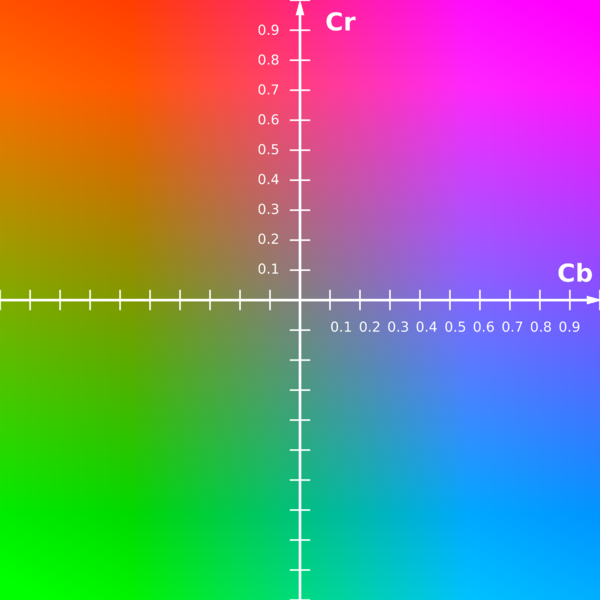
\includegraphics[width=0.7\linewidth]{theory/img/ycrcb_representation}
	\caption{Площина CbCr при Y = 0.5}
	\label{fig:ycrcb_representation}
\end{figure}

В комп'ютерній графіці часто YCrCb покоординатно переводять з відрізка $[0,1]$ у множину $[0,...,255]$ щоб кожну координату зберігати як беззнакове ціле число розміром 1 байт. Звісно це вносить деякі похибки, проте в такому форматі легче працювати з кольором.